\documentclass[../classical_mechanics.tex]{subfiles}

\begin{document}

    \section{Introduction}
        \paragraph{}
        Mechanics is the study of how things move; from the Earth orbiting the Sun, to a ball rolling down a hill, to an electron in a cathode ray tube.
        The modern formulation of classical mechanics was first developed in the 17\ts{th} and 18\ts{th} centuries by European natural philosophers like Galileo and Newton, who based their ideas on previous theories like those from ancient Greece.
        It was then reformulated in the 19\ts{th} century by French mathematicians such as Lagrange, Poisson and Liouville, as well as Hamilton, whose developments paved the way for the innovations of the 20\ts{th} century, when it was realised that classical mechanics cannot accurately describe objects travelling close to the speed of light or objects that are extremely small (on an atomic scale).
        These discoveries led to the development of relativistic mechanics and quantum mechanics, for which the advanced Lagrangian and Hamiltonian formalisms serve as a mathematical basis.

        \paragraph{}
        In this text we will be studying the Newtonian formulation of classical mechanics, which is still used today not only as a teaching method, but also as a tool in research.
        The Lagrangian and Hamiltonian formalisms come into their own for advanced problems, but can be quite unwieldy for the simple systems that we will be describing the motion of.
        One may wonder why we still study classical mechanics if it has been proven to be obsolete in some areas.
        The answer is that there are still many real-life systems which are best described using a classical description.
        It is also a great opportunity to become familiar with the language of vector calculus while studying examples which are relevant to real life.
        Without further ado, let us dive in to how we describe the world in mechanics.
        % talk about predicting the future, determinism, reversibility

    \section{Motion in One Dimension}\label{sec:motion-in-1d}
        \paragraph{}
        No doubt you will have noticed that the world is three dimensional.
        However it is certainly beneficial to study motion in a simplified setting before extending our ideas to the full 3D application.
        In Newtonian mechanics, we label each point in space with a \textbf{continuous variable} $x$, and we define an origin where $x=0$.
        This defines our \textbf{coordinate system}.
        We can describe the motion of an object by writing its position $x$ as a function of a continuous parameter $t$, which describes the passage of time from a reference point $t=0$.
        \begin{definition}
            The \textbf{trajectory} of an object is a function $x(t)$ where $t,x(t)\in\RR$. $x(t_0)=x_0$ describes the position of the object $x_0$ at some time $t_0$.
        \end{definition}

        \paragraph{}
        In classical mechanics, time evolves as the same rate for the whole universe.
        Our choice of coordinate system together with our choice of reference point for time is called a \textbf{reference frame}.
        By choosing our reference frame cleverly, we can often simplify problems.
        For example, if we were studying a block sliding down a slope, we could simplify the problem by rotating our coordinate system so that the $x$ axis lies parallel to the slope.
        In general, it is often best to align the $x$ axis with the direction of motion.
        \begin{definition}
            The \textbf{displacement} of an object is the difference in positions between two times $t_1$ and $t_2>t_1$. In one dimension:
            \begin{equation}
                \Delta x=x(t_2)-x(t_1)=x_2-x_1.
            \end{equation}
            If $x(0)=x_0$, then the \textbf{total displacement} of an object as a function of time is given by
            \begin{equation}
                s(t)=x(t)-x_0.
            \end{equation}
        \end{definition}
        The \textbf{distance} travelled by an object between $t_1$ and $t_2$ is given by the magnitude of displacement,
        \begin{equation}
            \mathrm{distance}=\abs{\Delta x}=\abs{x(t_2)-x(t_1)}=\abs{x_2-x_1}.
        \end{equation}
        In general, distance $\neq$ displacement.
        This is because displacement is a \textbf{vector} quantity, meaning it has direction and magnitude, whereas distance is a \textbf{scalar} quantity.
        In one dimension, the only difference between vector and scalar quantities is that vector quantities are \textbf{signed}.
        The distinction becomes greater in more dimensions when vector quantities are actually represented as vectors.
        \begin{definition}
            The \textbf{instantaneous velocity}, or just the \textbf{velocity} of an object is defined as the rate of change of the object's position with respect to time, or simply the derivative.
            \begin{equation}
                v(t)=\lim_{\Delta t\to0}\frac{x(t+\Delta t)-x(t)}{\Delta t}=\dv{x(t)}{t}.
            \end{equation}
        \end{definition}
        Velocity is also a vector quantity.
        The corresponding scalar quantity is \textbf{speed}, defined as the magnitude of velocity,
        \begin{equation}
            \mathrm{speed}=\abs{v(t)}.
        \end{equation}
        The \textbf{average velocity} of an object in a time interval $\Delta t=t_2-t_1$ is given by the displacement over the time interval, or also the time average of the velocity (which must be computed with an integral since it is a continuous property).
        \begin{equation}
            \bar{v}=\frac{\mathrm{total\ displacement}}{\mathrm{total\ time}}=\frac{\Delta x}{\Delta t}=\frac{1}{\Delta t}\int_{t_1}^{t_2}v(t)\dd{t}.
        \end{equation}
        Meanwhile, the \textbf{average speed} is given by
        \begin{equation}
            \overline{\mathrm{speed}}=\frac{\mathrm{total\ distance}}{\mathrm{total\ time}}=\frac{1}{\Delta t}\int_{t_1}^{t_2}\abs{v(t)}\dd{t}.
        \end{equation}
        Here, we may identify
        \begin{equation}\label{eq:total-disp}
            \Delta x=\int_{t_1}^{t_2}v(t)\mathrm{d}t,\quad \mathrm{total\ distance}=\int_{t_1}^{t_2}\abs{v(t)}\dd{t}.
        \end{equation}
        If the object is travelling at constant velocity, then the integral is trivial and we recover (setting $t_1=0$) the equation that you probably learned in school,
        \begin{equation}
            \mathrm{distance}=\mathrm{speed}\times\mathrm{time}.
        \end{equation}
        \begin{definition}
            The \textbf{instantaneous acceleration}, or just the \textbf{acceleration} of an object is defined as the rate of change of the object's velocity with respect to time.
            \begin{equation}
                a(t)=\lim_{\Delta t\to0}\frac{v(t+\Delta t)-v(t)}{\Delta t}=\dv{v(t)}{t}=\dv[2]{x(t)}{t}.
            \end{equation}
        \end{definition}
        Likewise, the \textbf{average acceleration} of an object in a time interval $\Delta t$ is
        \begin{equation}\label{eq:average-acc}
            \bar{a}=\frac{\Delta v}{\Delta t}=\frac{1}{\Delta t}\int_{t_1}^{t_2}a(t)\dd{t}.
        \end{equation}

    \section{Constant Acceleration}\label{sec:suvat}
        \paragraph{}
        When the acceleration of an object is constant, we can derive some useful equations for simple motion.
        Starting from equation \ref{eq:average-acc} above,
        \begin{align*}
            \Delta v&=\int_{t_1}^{t_2}a\dd{t}\\
            \implies v_2-v_1&=a\cdot(t_2-t_1),
        \end{align*}
        now setting $t_1=0,t_2=t,v_1=v(0)=u,v_2=v(t)$, we get
        \begin{equation}\label{eq:suvat-1}
            v(t)=u+at,
        \end{equation}
        where $u$ is the initial velocity of the object.
        Now we substitute equation \ref{eq:suvat-1} into equation \ref{eq:total-disp} to get
        \begin{align*}
            \Delta x&=\int_{t_1}^{t_2}(u+at)\dd{t}\\
            \implies x_2-x_1&=u\cdot(t_2-t_1)+\frac{1}{2}a\cdot(t_2^2-t_1^2).
        \end{align*}
        Setting $t_1=0,t_2=t,x_1=x(0)=x_0,x_2=x(t)$ like before and recalling $s(t)=x(t)-x_0$, we get
        \begin{equation}\label{eq:suvat-2}
            s(t)=ut+\frac{1}{2}at^2.
        \end{equation}
        Finally, squaring equation \ref{eq:suvat-1} and substituting in equation \ref{eq:suvat-2} gives
        \begin{equation}\label{eq:suvat-3}
            v^2(t)=u^2+2as(t).
        \end{equation}
        Equations \ref{eq:suvat-1}, \ref{eq:suvat-2}, and \ref{eq:suvat-3} are known as the SUVAT equations, you probably learned them in school.
        They are the \textbf{equations of motion} for a object under constant acceleration, i.e. all problems involving constant acceleration in a straight line are solved by them.
        \begin{example}
            Ball thrown in the air % TODO: write this
        \end{example}

        Now let's do some examples where we do not have constant acceleration.
        % TODO: add example for intuition with graphs, (how do tell if something is accelerating/ increaasing acceleration, etc.)
        % inflection points => curvature = acceleration = 0
        \begin{example}
            Car accelerating then decelerating % TODO: write this
            \begin{equation*}
                v(t)=-\frac{1}{2}t^4+3t^3
            \end{equation*}
        \end{example}
        \begin{example}
            Block sliding down a hill (no friction) % TODO: write this
        \end{example}

    \section{Motion in More than One Dimension}\label{sec:motion-in-2-3d}
        \paragraph{}
        As alluded to in section~\ref{sec:motion-in-1d} above, motion in more than one dimension is a straightforward generalisation of what we have learned so far.
        This is because the set of all points in 3D space forms a \textbf{vector space}, called $\RR^3$, so we can pick 3 \textbf{orthogonal} axes and an origin to use as our coordinate system and define three basis vectors to span all of space.
        In \textbf{cartesian} coordinates, which are the most commonly used system to label points in 3D space, we label the axes $x$, $y$ and $z$, and choose the unit vectors $\ihat$, $\jhat$ and $\khat$ to point along each axis respectively.
        \begin{figure}[H]
            \centering
            \begin{tikzpicture}[scale=2]
                \draw[<->] (0,1) |- (1,0);
                \draw[->] (0,0) -- (0.8,0.4);
                \node[right] at (1,0) {$x$};
                \node[above right] at (0.8,0.4) {$y$};
                \node[above] at (0,1) {$z$};

                \draw[<->,thick] (0,0.4) |- (0.4,0);
                \draw[->,thick] (0,0) -- (0.32,0.16);
                \node[below right] at (0.4,0) {$\ihat$};
                \node[above] at (0.32,0.16) {$\jhat$};
                \node[above left] at (0,0.4) {$\khat$};
            \end{tikzpicture}
        \end{figure}

        \paragraph{}
        A general vector in 3D cartesian coordinates is represented by a sum of components along each direction.
        \begin{equation}
            \vec{A}=A_x\ihat+A_y\jhat+A_z\khat.
        \end{equation}
        In 2D (where we don't have a $z$ component), there is a simple way to calculate the components using the angle that the vector makes with the $x$ axis.
        \begin{figure}[H]
            \centering
            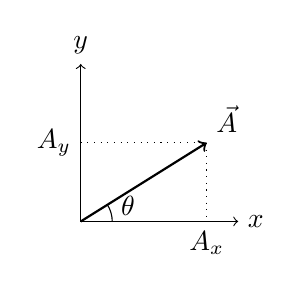
\begin{tikzpicture}[scale=2]
                \draw[<->] (0,1) |- (1,0);
                \node[right] at (1,0) {$x$};
                \node[above] at (0,1) {$y$};

                \draw[->,thick] (0,0) -- (0.8,0.5);
                \node[above right] at (0.8,0.5) {$\vec{A}$};
                \draw (0.2,0) arc [radius=0.2, start angle=0, end angle=32];
                \node at (0.3,0.1) {$\theta$};

                \draw[dotted] (0,0.5) -- (0.8,0.5) -- (0.8,0);
                \node[left] at (0,0.5) {$A_y$};
                \node[below] at (0.8,0) {$A_x$};
            \end{tikzpicture}
        \end{figure}
        First, note that the length of the vector is given by Pythagoras' theorem:
        \begin{equation}\label{eq:2d-polar-length}
            \abs{\vec{A}}=\sqrt{A_x^2+A_y^2}.
        \end{equation}
        Then, using trigonometry, the components $A_x$ and $A_y$ are given by
        \begin{align}
            A_x&=\abs{\vec{A}}\cos\theta\label{eq:2d-polar-x-component}\\
            A_y&=\abs{\vec{A}}\sin\theta\label{eq:2d-polar-y-component}.
        \end{align}
        We also have a relation for the angle:
        \begin{equation}
            \tan\theta=\frac{A_y}{A_x}\label{eq:2d-polar-theta}.
        \end{equation}
        In 3D we need two angles to describe the direction of a vector, so the relations become slightly more complicated.
        % TODO: write these

        \paragraph{}
        Note that it is important that our basis vectors are \textbf{orthonormal}, meaning both orthogonal and of unit length, as this means we have the relations
        \begin{align}
            &\abs{\ihat}=\abs{\jhat}=\abs{\khat}=1\label{eq:basis-vec-magnitude}\\
            &\ihat\cdot\ihat=\jhat\cdot\jhat=\khat\cdot\khat=1\label{eq:basis-vec-normal}\\
            &\ihat\cdot\jhat=\jhat\cdot\khat=\khat\cdot\ihat=0\label{eq:basis-vec-ortho}.
        \end{align}
        If these results were not true, then some of the mathematics we will do later on (involving dot and cross products) would become much more complicated than it needs to be.
        \begin{definition}
            The \textbf{trajectory} of an object in three dimensions is a vector-valued function $\vec{r}(t)$ where $t\in\RR$, $\vec{r}(t)\in\RR^3$.
            We write
            \begin{equation}
                \vec{r}(t)=x(t)\ihat+y(t)\jhat+z(t)\khat
            \end{equation}
            in cartesian coordinates, where $x(t)$, $y(t)$ and $z(t)$ are the 1D trajectories of the object along each axis.
            For example, if $\vec{r}(t_0)=\vec{r}_0=x_0\ihat+y_0\jhat+z_0\khat$, then the object is located at position $x_0$ along the $x$ axis, $y_0$ along the $y$ axis and $z_0$ along the $z$ axis.
            $\vec{r}(t)$ is known as the \textbf{position vector}.
        \end{definition}
        At this point it is worth introducing a new notation which will simplify our expressions going forward.
        We will represent a time derivative of a quantity by simply writing a dot above the letter, and put two dots for a second derivative.
        \begin{equation}
            \dot{x}=\dv{x}{t},\quad\ddot{x}=\dv[2]{x}{t},
        \end{equation}
        i.e. $\dot x$ represents velocity and $\ddot x$ represents acceleration.
        The notation is due to Newton and so it is fitting that we use it a lot in mechanics.
        We have also stopped notating dependence on time explicitly for brevity and to reduce clutter in the notation.
        \begin{definition}
            Just as in one dimension.
            The velocity is defined as the time derivative of position.
            \begin{equation}
                \vec{v}=\dot{\vec{r}}=\dv{\vec{r}}{t}=\dv{x}{t}\ihat+\dv{y}{t}\jhat+\dv{z}{t}\khat=\dot{x}\ihat+\dot{y}\jhat+\dot{z}\khat.
            \end{equation}
            Sometimes we denote $\dot{x}$, $\dot{y}$ and $\dot{z}$ as $v_x$, $v_y$ and $v_z$ respectively.
        \end{definition}
        \begin{definition}
            Likewise, acceleration is the time derivative of velocity, or the second time derivative of position.
            \begin{equation}
                \vec{a}=\ddot{\vec{r}}=\dv{v}{t}=\dv[2]{r}{t}=\ddot{x}\ihat+\ddot{y}\jhat+\ddot{z}\khat.
            \end{equation}
            Sometimes $\ddot{x}$, $\ddot{y}$ and $\ddot{z}$ are called $a_x$, $a_y$ and $a_z$.
        \end{definition}
        The key insight is that motion in 3D Cartesian coordinates is simply a superposition of three one-dimensional motions.
        Because of this, it is possible (and convenient) for simple problems to ignore the vector nature of the problem and just treat motion along each axis as a separate scalar problem.
        
        \paragraph{}
        Suppose we want to take the dot product of two vectors.
        We can compute it by writing each vector as a sum of components and then multiplying out the brackets.
        Going through the steps in cartesian coordinates, we get
        \begin{align}
            \vec{A}\cdot\vec{B}&=(A_x\ihat+A_y\jhat+A_z\khat)\cdot(B_x\ihat+B_y\jhat+B_z\khat)\\
            &\begin{aligned}
                &=A_x\ihat\cdot B_x\ihat+A_x\ihat\cdot B_y\jhat+A_x\ihat\cdot B_z\khat+A_y\jhat\cdot B_x\ihat+A_y\jhat\cdot B_y\jhat+A_y\jhat\cdot B_z\khat\\
                &\quad+A_z\khat\cdot B_x\ihat+A_z\khat\cdot B_y\jhat+A_z\khat\cdot B_z\khat
            \end{aligned}\\
            &=A_xB_x\ihat+A_yB_y\jhat+A_zB_z\khat.
        \end{align}
        The last step only follows because the basis vectors are \textbf{orthonormal}.
        This is because the terms with two different basis vectors dotted together vanish (equation~\ref{eq:basis-vec-ortho}) and the terms with two of the same basis vector become just the coordinates multiplied together (equation~\ref{eq:basis-vec-normal}).
        All the coordinate systems we have dealt with so far have an orthonormal basis because of this fact.

    \section{Forces}
        \paragraph{}
        Now we know how to describe the motion of an object and changes in the motion (kinematics), but we still don't know how to describe \textit{why} the motion of an object changes (dynamics).
        This is the focus of this section.

        \paragraph{}
        A force is some influence on an object that changes the object's motion.
        In classical mechanics, we describe forces as vectors and denote a generic force with the symbol $F$.
        The exact dynamics of how forces affect motion are described in Newton's laws of motion, which we will write now.
        In the following the symbol $F$ stands for the sum of all forces acting on the object, otherwise known as the \textbf{net force}.
        \begin{definition}[Newton's First Law]\label{def:newton-1}
            An object moving with constant velocity $v$, will stay at the same constant velocity unless acted upon by a force.
            In other words:
            \begin{equation}
                v=\text{const.}\iff F=0.
            \end{equation}
            Note that this includes an object at rest, which has velocity $v=0$.
        \end{definition}
        Mass is defined as an objects resistance to acceleration.
        In order words, a more massive object will accelerate slower relative to a less massive object when under the influence of identical forces.
        This is quantified by Newton's Second Law.
        \begin{definition}[Newton's Second Law]\label{def:newton-2}
            The net force on the object is equal to the object's mass times the object's acceleration.
            \begin{equation}
                F=ma.
            \end{equation}
            Note that force is always parallel to acceleration.
        \end{definition}
        Since acceleration is the second derivative of position, we can write Newton's Second Law as
        \begin{equation}
            F(t)=m\dv[2]{x(t)}{t},
        \end{equation}
        which is a differential equation for $x(t)$.
        This is known as an \textbf{equation of motion}, and all classical mechanics problems boil down to solving the equation of motion to obtain the trajectory of the object.
        \begin{example}
            Suppose an object is acted upon by a constant force $F_0$, then we align the $x$ axis with the direction of the force and the equation of motion is
            \begin{equation*}
                \dv[2]{x(t)}{t}=\frac{F_0}{m}.
            \end{equation*}
            This is a very easy differential equation to solve.
            Integrating twice, we get
            \begin{align*}
                &\dv{x(t)}{t}=\int\dv[2]{x(t)}{t}=v_0+\frac{F_0}{m}t\\
                &x(t)=\int\dv{x(t)}{t}=x_0+v_0t+\frac{F_0}{2m}t^2,
            \end{align*}
            where $v_0=v(0)$ and $x_0=x(0)$ as before.
            Note that comparing to equation \ref{eq:suvat-2}, we can identify $a=\frac{F_0}{m}$ i.e. acceleration is constant, which is consistent with what we developed before.
        \end{example}
        It is important to note that Newton's Laws of Motion are only valid in \textbf{inertial reference frames}, which are reference frames travelling at a constant velocity $v$.
        If we are in a nonintertial reference frame, i.e. one that is accelerating, and we try to apply Newton's Laws, we will encounter odd things such as phantom forces which have no source.
        One way to test if we are in an inertial frame or not us by using Newton's First Law.
        If an object accelerates while under the influence of no forces, then our reference frame must be noninertial.
        \begin{definition}[Newton's Third Law]\label{def:newton-3}
            When two objects interact with each other, the forces on each object due to the other are \textbf{equal in magnitude} and \textbf{opposite in direction}.
            In other words, if object $A$ exerts a force $F_{A\to B}$ on object $B$, then object $B$ exerts a force $F_{B\to A}$ on object $A$ and we may write
            \begin{equation}
                F_{A\to B}=-F_{B\to A}.
            \end{equation}
            These two forces are then known as a ``Newton (III) pair''.
        \end{definition}

        \paragraph{}
        Force is a vector quantity, so in more than dimension it can be decomposed into multiple components which are the forces along each axis.
        In three dimensions, Newton's Second Law is
        \begin{align*}
            \vec{F}(t)&=F_x(t)\ihat+F_y(t)\jhat+F_z(t)\khat\\
            &=ma_x(t)\ihat+ma_y(t)\jhat+ma_z(t)\khat \\
            &=m\vec{a}=m\ddot{\vec{r}}.
        \end{align*}

        % TODO: talk about gravity and normal force
        % TODO: talk about free-body diagrams
        We can now solve any problem in classical mechanics.

    \section{Projectile Motion}
        \paragraph{}
        Let's now look at a concrete example of an experiment which will bring together everything we have looked at in this chapter.
        Suppose we have a cannon situated at the origin which shoots a projectile with a fixed initial velocity $\vec{v}_0$ which makes an initial angle $\theta$ relatitive to the ground.
        Can we work out how far the projectile will fly and what its flight time is?
        % TODO: add diagram
        \paragraph{}
        This is going to be a 2D problem as we have two axes of motion.
        We shall label the horizontal direction that the cannon is shooting along the $x$ axis and the vertical direction the $y$ axis.
        As stated in the problem, the cannon is located at the origin.
        We can now write the initial velocity as
        \begin{equation}
            \vec{v}_0 = v_0\cos(\theta)\ihat + v_0\sin(\theta)\jhat,
        \end{equation}
        where $v_0=\abs{\vec{v}_0}$.
        Ignoring air resistance, there are no forces acting on the projectile in the $x$ direction.
        By Newton's second law this means that $a_x=0$ and we can immediately write
        \begin{equation}
            x(t) = v_0\cos(\theta)t,
        \end{equation}
        using the SUVAT equation \ref{eq:suvat-2}.
        In the $y$ direction, the only force acting on the projectile is the constant force of gravity, so Newton's second law tells us
        \begin{equation}
            F_y = -mg = ma_y.
        \end{equation}
        Hence, we have
        \begin{equation}
            y(t) = v_0\sin(\theta)t - \frac{1}{2}gt^2,
        \end{equation}
        again by equation \ref{eq:suvat-2}.

        \paragraph{}
        Now, the time of flight $t_f$ will be given when $y(t_f)=0$.
        Solving for this, we get
        \begin{align}
            y(t_f) = &v_0\sin(\theta)t_f - \frac{1}{2}gt_f^2 = 0\\
            &v_0\sin(\theta)t_f = \frac{1}{2}gt_f^2\\
            &t_f = \frac{2v_0\sin(\theta)}{g}.
        \end{align}
        Let's consider briefly if this answer makes physical sense.
        If the initial speed of the projectile $v_0$ was higher, then the flight time would be longer.
        Additionally, for a fixed initial speed, a projectile fired at a higher angle would have a longer flight time because more of the initial velocity was aimed along the vertical direction.
        On the other hand, if gravity was stronger, the projectile would fall to the ground faster and the flight time would be shorter.

        \paragraph{}
        Finally, the range of the projectile is given by
        \begin{align}
            x_f = x(t_f) &= v_0\cos(\theta)t_f\\
            &= \frac{2v_0^2\sin(2\theta)}{g}.
        \end{align}
        So the maximum range is given when $\theta=\frac{\pi}{4}$.

        % TODO: include a discussion of drag

        \begin{example}
            A motorcyclist is doing a stunt jump between two buildings.
            If the buildings are separated by a distance $d$ and have a vertical height difference $h$, what is the minimum velocity the motorcyclist needs to make the jump?
            % TODO: complete this example
        \end{example}

    \section{Friction}
        \paragraph{}
        Friction is a very complicated process which occurs on a miroscopic scale, so in order to model in on a macroscopic scale we must use simplified empirical laws.
        In general, friction is a force which opposes change in motion. Hence if a force is applied parallel to a surface, then the frictional force will be antiparallel to this, perpendicular to the normal force.

        \paragraph{}
        Satic friction appears when two objects are motionless with respect to one another.
        If a force is applied between the two objects and they don't move, there must be a frictional force opposing the motion.
        % TODO: add a diagram
        \begin{equation}
            \vec{f}_s=-\vec{F}_{app}.
        \end{equation}
        As the applied force gets larger, the static friction must get larger to preserve equilibrium, until a maximum limit is reached and the object starts moving.
        \begin{definition}
            The maximum magnitude of \textbf{static friction} is given by
            \begin{equation}
                f_{s,max}=\mu_s\abs{\vec{N}}.
            \end{equation}
            Hence,
            \begin{equation}
                0\leq\abs{\vec{f}_s}\leq f_{s,max}.
            \end{equation}
        \end{definition}

        \paragraph{}
        Kinetic friction opposes the motion of two surfaces sliding against each other.
        \begin{definition}
            \textbf{Kinetic friction} is given by
            \begin{equation}
                \vec{f}_k=-\mu_k\abs{\vec{N}}\uvec{v}.
            \end{equation}
        \end{definition}
        % TODO: include discussion of critical angle
        \begin{example}
            Find the stopping distance of a block sliding down a slope.
            % TODO: write this
        \end{example}
        \begin{example}
            Three blocks --- A, B, and C --- are connected over a slope by massless inextensible ropes going through frictionless pulleys.
            Blocks A and B both have a weight of $\qty{25}{\newton}$ a coefficient of kinetic friction of $\mu_k=0.35$.
            The angle of the slope is $\ang{30}$ and block C is falling with constant velocity.
            What is the weight of block C?
            \begin{figure}[H]
                \centering
                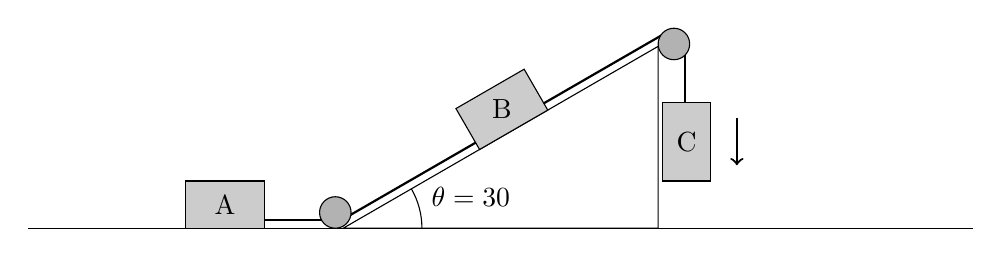
\begin{tikzpicture}[scale=2]
                    % triangle
                    \draw (0,0) -- (6,0);
                    \draw (2,0) -- (4,0) -- (4,1.155) -- cycle;
                    \draw (2.5,0) arc [radius=0.5, start angle=0, end angle=30];
                    \node[right] at (2.5,0.2) {$\theta=\ang{30}$}; 

                    % blocks
                    \draw[fill=black!20] (1,0) rectangle (1.5,0.3);
                    \node at (1.25, 0.15) {A};
                    \begin{scope}[shift={(2,0)},rotate=30]
                        \draw[fill=black!20] (1,0) rectangle (1.5,0.3);
                        \node at (1.25,0.15) {B};
                    \end{scope}
                    \draw[shift={(4.03,0.8)},fill=black!20] (0,0) rectangle (0.3,-0.5);
                    \draw[shift={(4.03,0.8)}] (0.15,-0.25) node {C};
                    \draw[->,thick] (4.5,0.7) -- (4.5,0.4);

                    % ropes
                    \draw[thick] (1.5,0.05) -- (1.95,0.05);
                    \begin{scope}[shift={(2,0)},rotate=30]
                        \draw[thick] (0,0.05) -- (1,0.05);
                        \draw[thick] (1.5,0.05) -- (2.4,0.05);
                    \end{scope}
                    \draw[thick] (4.17,1.17) -- (4.17,0.8);

                    % pulleys
                    \draw[fill=black!30] (1.95,0.1) circle [radius=0.1];
                    \draw[fill=black!30] (4.1,1.17) circle [radius=0.1];
                    
                \end{tikzpicture}
            \end{figure}
            
            \paragraph{}
            We will start to solve this problem by drawing free-body diagrams for all the blocks.
            In each diagram, we will orient the $x$-axis along the direction of motion.
            \begin{figure}[H]
                \centering
                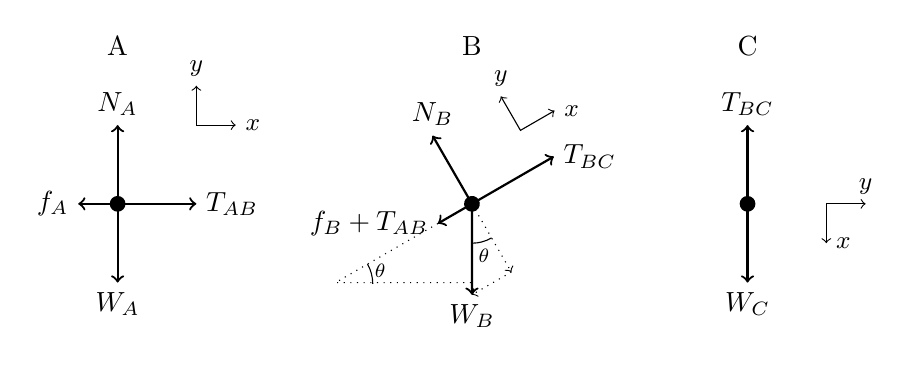
\begin{tikzpicture}
                    % block A
                    \begin{scope}[shift={(-4,0)}]
                        \fill (0,0) circle [radius=0.1];
                        \node at (0,2) {A};
                        \draw[<->,thick] (-0.5,0) -- (1,0);
                        \draw[<->,thick] (0,-1) -- (0,1);
                        \node[left] at (-0.5,0) {$f_A$};
                        \node[right] at (1,0) {$T_{AB}$};
                        \node[above] at (0,1) {$N_A$};
                        \node[below] at (0,-1) {$W_A$};

                        \begin{scope}[shift={(1,1)},scale=0.5,font=\small]
                            \draw[<->] (0,1) |- (1,0);
                            \node[right] at (1,0) {$x$};
                            \node[above] at (0,1) {$y$};    
                        \end{scope}
                    \end{scope}

                    % block B
                    \begin{scope}[shift={(0.5,0)}]
                        \node at (0,2) {B};
                        \begin{scope}[rotate=30]
                            \fill (0,0) circle [radius=0.1];
                            \draw[<->,thick] (0,1) -- (0,0) -- (1.2,0);
                            \draw[<-,thick] (-0.5,0) -- (0,0);
                            \draw[->,thick] (0,0) -- (-0.577,-1);
                            \draw[->,dotted] (0,0) -- (0,-1);
                            \draw[->,dotted] (0,-1) -- (-0.577,-1);
                            \draw[dotted,rotate=-30] (0,0) -- (0,-1) -- (-1.732,-1) -- cycle;
                            \draw (-1.532,0) arc [radius=0.5, start angle=0, end angle=-30];
                            \node[font=\scriptsize] at (-1.432,-0.15) {$\theta$};
                            \draw (0,-0.5) arc [radius=0.5, start angle=270, end angle=240];
                            \node[font=\scriptsize] at (-0.2,-0.65) {$\theta$};
                            \node[above] at (0,1) {$N_B$};
                            \node[right] at (1.2,0) {$T_{BC}$};
                            \node[left] at (-0.5,0) {$f_B+T_{AB}$};
                            \node[below] at (-0.577,-1) {$W_B$};

                            \begin{scope}[shift={(1,0.5)},scale=0.5,font=\small]
                                \draw[<->] (0,1) |- (1,0);
                                \node[right] at (1,0) {$x$};
                                \node[above] at (0,1) {$y$};    
                            \end{scope}
                        \end{scope}
                    \end{scope}

                    % block C
                    \begin{scope}[shift={(4,0)}]
                        \fill (0,0) circle [radius=0.1];
                        \node at (0,2) {C};
                        \draw[<->,thick] (0,1) -- (0,-1);
                        \node[above] at (0,1) {$T_{BC}$};
                        \node[below] at (0,-1) {$W_C$};

                        \begin{scope}[shift={(1,0)},scale=0.5,rotate=-90,font=\small]
                            \draw[<->] (0,1) |- (1,0);
                            \node[right] at (1,0) {$x$};
                            \node[above] at (0,1) {$y$};    
                        \end{scope}
                    \end{scope}
                \end{tikzpicture}
            \end{figure}
            Since the ropes are inextensible, the tension throughout them must be uniform.
            Therefore all the blocks must be moving together at the same speed.
            This speed is constant, so Newton's second law tells us that the resultant forces along both axes, $\Sigma F_x$ and $\Sigma F_y$, must be zero for all three blocks.
            Looking at the diagram for block C, this tells us that $W_C$, the weight of block C, is equal in magnitude to $T_{BC}$, the tension in the rope connecting B and C.

            From the diagram for block B we have
            \begin{align}
                \Sigma F_y&=N_B-W_B\cos\theta=0\\
                \implies N_B&=W_B\cos\theta
            \end{align}
            and
            \begin{align}
                \Sigma F_x&=T_{BC}-(f_B+T_{AB})-W_B\sin\theta=0\\
                \implies T_{BC}&=f_B+T_{AB}+W_B\sin\theta\\
                &=\mu_k W_B\cos\theta+T_{AB}+W_B\sin\theta,
            \end{align}
            from block A we get
            \begin{align}
                \Sigma F_y&=N_A-W_A=0\\
                \implies N_A&=W_A
            \end{align}
            and
            \begin{align}
                \Sigma F_x&=T_{AB}-f_A=0\\
                \implies T_{AB}&=f_A=\mu_k N_A\\
                &=\mu_k W_A.
            \end{align}
            Combining all these results, we get
            \begin{align}
                W_C&=T_{BC}\\
                &=\mu_k W_B\cos\theta+W_B\sin\theta+\mu_k W_A\\
                &=\qty{7.58}{\newton}+\qty{12.5}{\newton}+\qty{8.75}{\newton}\\
                &=\qty{28.83}{\newton}.
            \end{align}

            \paragraph{}
            Now, imagine if the rope between blocks A and B is cut.
            What will happen to block C?

            \paragraph{}
            With both blocks A and B providing block C with enough friction to balance gravity, it seems that if we remove block A then there will no longer be enough resistance and block C will have to accelerate downwards.
            We can try calculating the acceleration and find out if our hypothesis is correct.
            The forces on blocks B and C are all the same except that we no longer have $T_{AB}$.
            Thus for block C we get
            \begin{align}
                \Sigma F_x&=W_C-T_{BC}=\frac{W_C}{g}a,\\
            \end{align}
            and for block B we get
            \begin{align}
                \Sigma F_x&=T_{BC}-f_B-W_B\sin\theta=\frac{W_B}{g}a\\
                \implies T_{BC}&=\mu_k W_B\cos\theta+W_B\sin\theta+\frac{W_B}{g}a.
            \end{align}
            Combining these, we get
            \begin{align}
                W_C-\frac{W_C}{g}a&=\mu_k W_B\cos\theta+W_B\sin\theta+\frac{W_B}{g}a\\
                \frac{(W_C+W_B)}{g}a&=W_C-W_B\sin\theta-\mu_k W_B\cos\theta\\
                a&=\frac{W_C-W_B(\sin\theta+\mu_k\cos\theta)}{W_C+W_B}g\\
                &=\qty{1.59}{\metre\per\square\second}.
            \end{align}
            This acceleration is nonzero and positive, which indicates that block C does indeed accelerate downwards as we thought.
        \end{example}

    \section{Gravitation}
        \paragraph{}
        Aside from inventing classical mechanics and calculus, Isaac Newton's most well-known contribution to science is his discovery of the universal law of gravitation.
        % TODO: write more about how it was derived
        % TODO: include a proper definition
        If we consider two objects, one of which is located at the origin, then the gravitational force between the two bodies has magnitude
        \begin{equation}
            F=\frac{Gm_1m_2}{r^2}.
        \end{equation}
        % TODO: include diagram for this
        In vectorial form, these forces form a Newton III pair.
        \begin{align}
            \vec{F}_{1\to2}&=-\frac{Gm_1m_2}{\abs{\vec{r}_{1\to2}}^3}\vec{r}_{1\to2}\\
            \vec{F}_{2\to1}&=-\frac{Gm_1m_2}{\abs{\vec{r}_{2\to1}}^3}\vec{r}_{2\to1}=\frac{Gm_1m_2}{\abs{\vec{r}_{1\to2}}^3}\vec{r}_{1\to2}=-\vec{F}_{2\to1},
        \end{align}
        where $\vec{r}_{1\to2}=\vec{r}_{2\to1}=\vec{r}_2-\vec{r}_1$.
        
        \paragraph{}
        Consider an object of mass $m$ near the surface on the Earth.
        The radius of the Earth is very large so we can approximate the distance between the Earth and the object as simply the radius of the Earth.
        The gravitational force which the Earth exerts on the object is given by
        \begin{equation}
            F_G\approx\frac{GM_\text{Earth}}{R_\text{Earth}^2}m=mg,
        \end{equation}
        where $g=\frac{GM_\text{Earth}}{R_\text{Earth}^2}$.
        Thus we have recovered the weight force that we have been using for the force due to gravity.
        If the height of the object is so large that the approximation no longer holds, then $g$ depends on the height $R_\text{Earth}+h=r$.
        This is the same as the general case, the force only depends on the distance between the centre of the Earth and the object.
        Now consider the case where the object is \textit{below} the surface of the Earth.
        In this case, the mass of the Earth depends on the distance between the centre and the object.
        The mass enclosed within a radius $r$ is given by the density multiplied by the enclosed volume:
        \begin{equation}
            M(r)=\frac{4}{3}\rho\pi r^3.
        \end{equation}
        If we assume that the density of the Earth is constant, then it is given by the total mass divided by total volume:
        \begin{equation}
            \rho=\frac{M_\text{Earth}}{\frac{4}{3}\pi R_\text{Earth}^3}.
        \end{equation}
        Thus, $g(r)$ is given by
        \begin{align}
            g(r)&=\frac{GM(r)}{r^2}=\frac{G}{r^2}\frac{M_\text{Earth}}{R_\text{Earth}^3}r^3\\
            &=\frac{GM_\text{Earth}}{R_\text{Earth}^3}r.
        \end{align}
        % TODO: include diagram of g(r)
        \begin{example}
            Calculate $g$ at the surface of Earth.
            % TODO: complete this example
        \end{example}
        
\end{document}
